\documentclass[12pt]{article} % On précise la taille de police, et le type de document (article, livre, beamer, …)
\usepackage[T1]{fontenc} % La police utilisée
\usepackage[utf8]{inputenc} % L'encodage du document
\usepackage[french]{babel} % Des options supplémentaires pour que le document soit en français (noms de sections, etc.)
\usepackage{geometry}
\geometry{hscale=0.80,vscale=0.80,centering} % Permet de définir les marges (ici 10% de chaque côté)
\usepackage{amsmath,amsfonts,amssymb} % Permet l'utilisation de différents symboles mathématiques
\usepackage{hyperref} % Insertion de liens URL
\usepackage{tabularray} % Gestion des tableaux
\usepackage{enumitem} % Options particulières pour enumerate
\usepackage{multirow} % Fusion de lignes dans un tableau
\usepackage{graphicx} % Pour insérer des images
\usepackage{tikz} % Pour faire des graphiques
\usetikzlibrary{automata} % Quelques options pour les automates

%%% Vous pouvez ignorer les commandes suivantes %%%
\usepackage{textcomp}
\newcommand{\tbs}{\textbackslash}
\let\oldleq\leq
%%%%%%%%%%%%%%%%%%%%%%%%%%%%%%%%%%%%%%%%%%%%%%%%%%%

%%% Quelques commandes pour des environnements théorème/remarques/etc. %%%
\usepackage{amsthm}

\newtheorem{theoreme}{Théorème}[section]
\newtheorem{corolaire}{Corolaire}[theoreme]

\theoremstyle{definition}
\newtheorem{definition}{Definition}[section]

\theoremstyle{remark}
\newtheorem*{remarque}{Remarque}
%%%%%%%%%%%%%%%%%%%%%%%%%%%%%%%%%%%%%%%%%%%%%%%%%%%%%%%%%%%%%%%%%%%%%%%%%%%

\setlength{\parindent}{15pt} % Fixe l'indentation en début de paragraphe
\setlength{\parskip}{10pt} % Fixe l'espacement entre paragraphes

%%% Les commandes données en exemples dans la suite du document %%%
\newcommand{\lra}{\longrightarrow}
\newcommand{\limite}[2]{\underset{#1 \rightarrow #2}{\lra}}
\renewcommand{\leq}{\leqslant}
%%%%%%%%%%%%%%%%%%%%%%%%%%%%%%%%%%%%%%%%%%%%%%%%%%%%%%%%%%%%%%%%%%%

%%% Environnement code %%%
\usepackage{listings}
\usepackage{xcolor}

\lstset{basicstyle=\ttfamily,
        keywordstyle=\color{teal},
        commentstyle=\color{gray},
        stringstyle=\color{violet},
        identifierstyle=\color{blue}}
%%%%%%%%%%%%%%%%%%%%%%%%%%

\begin{document}

\title{Présentation de l'utilisation de \LaTeX{}\footnote{À modifier avec le bon titre}}
\date{\today}
\author{Nathaniel Carré}

\maketitle

\section{Introduction}

\subsection{Présentation}

Contrairement à un logiciel comme Microsoft Word, \LaTeX{} ne permet pas de faire de l'édition WYSIWYG (\textit{what you see is what you get}), c'est-à-dire que dans un document d'édition, on ne voit pas le résultat qu'on va obtenir, mais un simple document texte avec différentes commandes, qu'on doit compiler pour obtenir le document final.

\subsection{Installation}

De manière similaire à l'utilisation des langages de programmation, il faut installer deux choses pour pouvoir travailler avec \LaTeX{} : une distribution \LaTeX{} et un éditeur de texte.

Pour la distribution, je recommande Texlive (\url{https://www.tug.org/texlive/}), qui est la plus répandue et disponible sur tous les systèmes d'exploitation.

Quelque soit le système d'exploitation, si vous tapez la commande \verb"texdoc lshort-fr" après avoir installé Texlive, cela lancera un pdf qui est un manuel d'introduction (184 pages) à \LaTeX{}. On y trouve des exemples bien plus détaillés que dans ce document.

Pour l'éditeur, vous avez un vaste choix. Le mien est Texmaker, mais contrairement aux distributions, le choix de l'éditeur fait moins l'unanimité.

\subsection{Compilation}

Une distribution \TeX{} contient généralement plusieurs compilateurs. Le plus répandu (que j'utilise) est \verb"pdflatex", mais il commence à devenir obsolète sur certains aspects. Le compilateur \verb"lualatex" est se répand de plus en plus et est une très bonne alternative. Attention, le résultat du pdf obtenu change selon le compilateur utilisé, voire peut échouer si des paquets ou polices sont manquants pour l'un des compilateurs.

La plupart des éditeurs standards de \LaTeX{} proposent différentes options de compilation.

\subsection{D'autres manières de travailler avec \LaTeX{}}

Il est possible de se passer de l'utilisation d'un éditeur et d'une distribution. On peut mentionner le site Overleaf, qui permet de faire de l'édition \LaTeX{} en ligne, ou la solution LyX qui permet de faire du \LaTeX{} en WYSIWYM (\textit{what you see is what you mean}, autrement dit de contrôler de manière un peu plus simple la structure du document, sans faire apparaître les commandes sous-jacentes, mais sans que l'éditeur ne représente non plus le résultat final.

\section{Structure d'un document \LaTeX{}}

Un fichier \LaTeX{} est composé d'une entête, dans laquelle on importe généralement les paquets nécessaires à la compilation, et on définit les caractéristiques du document. Le corps du document est encadré par :
\begin{verbatim}
\begin{document}

\end{document}
\end{verbatim}

\subsection{Commandes et environnements}

\LaTeX{} contient un grand nombre de commandes permettant de faire une mise en forme particulière, ou d'intégrer un symbole. Par exemple, l'affichage de \LaTeX{} se fait avec la commande \verb"\LaTeX{}".  L'affichage de \verb"\LaTeX{}" en police \verb"tt" (\textit{typewritter}, c'est-à-dire machine à écrire) se fait avec \verb|\verb"\LaTeX{}"|.

On remarque que les commandes commencent par une contre-oblique (backslash) \verb"\", qui est le caractère usuel d'échappement. La plupart des commandes sont suivies d'une paire d'accolades, entre lesquelles on peut mettre des arguments. Par exemple, \verb"\textit{typewritter}" écrira en italique \textit{typewritter}. Ce n'est pas systématique, comme par exemple l'environnement verbatim précédent, qui peut utiliser différents délimiteurs (c'est ce qui m'a permis d'écrire des accolades dans l'environnement), ou des commandes sans délimiteurs, comme par exemple \# qui s'écrit avec \verb"\#".

Une autre manière de gérer la mise en forme est la notion d'environnement. On peut voir cela comme une commande avec un très long argument. Un environnement est généralement encadré par :
\begin{verbatim}
\begin{environnement}

\end{environnement}
\end{verbatim}
\noindent comme c'était le cas pour l'environnement \verb"document". Il existe un très grand nombre d'environnements très pratiques, comme les tableaux, les figures, les dessins, etc.

\subsection{Entête}

Outre quelques caractéristiques de forme, l'entête peut contenir l'importation des paquets (les bibliothèques nécessaires à la compilation, qui contiennent des commandes toutes faites), ainsi que des commandes ou macro personnalisées.

L'importation de paquets se fait via la commande \verb"\usepackage{nom_du_paquet}". La plupart des paquets disponibles sont généralement accompagnés d'une documentation détaillant leur utilisation.

\begin{remarque}
On peut créer des alias pour de nouvelles commandes, ou pour renommer des commandes existantes. Il faut simplement imaginer que la commande remplace une séquence plus longue. Par exemple, on peut écrire \verb"\newcommand{\lra}{\longrightarrow}" si on veut raccourcir la commande pour obtenir $\lra$. On peut imaginer des choses plus complexes, voire sur plusieurs lignes.

On peut écrire \verb"\newcommand{\limite}[2]{\underset{#1 \rightarrow #2}{\lra}}"  (avec deux arguments), pour pouvoir taper \verb"\limite{n}{+\infty}" et obtenir $\limite{n}{+\infty}$.

On peut renommer une commande existante, par exemple \verb"\renewcommand{\leq}{\leqslant}" pour que \verb"\leq" affiche $\leq$ au lieu de $\oldleq$.
\end{remarque}

\subsection{Corps du document}

\subsubsection{Sections}

On peut structurer le document en séparant les parties, en utilisant les commandes :
\begin{verbatim}
\section{Nom de section}
\subsection{Nom de sous-section}
\subsection{Nom de sous-sous-section}

\section*{Nom de section non numérotée}
\end{verbatim}

Les versions étoilées existent aussi pour les sous-sections et sous-sous-sections. Il n'existe pas de \verb"\subsubsubsection". Il existe d'autres commandes pour d'autres classes que \verb"article" (comme \verb"\chapter").
\subsubsection{Espacements}
Les espacements répondent aux règles suivantes :
\begin{itemize}
\item les espaces consécutives sont ignorées au dela de la première ;
\item un retour à la ligne est ignoré ;
\item une ligne blanche intermédiaire marque un nouveau paragraphe, les lignes blanches au delà de la première sont ignorées ;
\item on peut forcer un retour à la ligne sans marquer de nouveau paragraphe avec \verb"\\". On peut enchaîner les \verb"\\" pour sauter plusieurs lignes ;
\item on peut forcer un retour à la ligne en forçant l'alignement du paragraphe avec \verb"\linebreak" ;
\item une espace simple peut être coupée à l'affichage par une fin de ligne. On peut éviter de couper en utilisant \texttt{\raisebox{0.5ex}{\texttildelow}} qui est le caractère d'espace insécable. Par exemple, si on écrit \texttt{les règles suivantes\raisebox{0.5ex}{\texttildelow}:}, le deux-points ne sera jamais séparé du mot « suivantes » ;
\item on peut forcer une nouvelle page avec \verb"\newpage".\\
\end{itemize}

Dans certains cas (figures, mathématiques, prise de tête sur une suite de commandes particulières), on peut vouloir rajouter des espacements horizontaux ou verticaux à la main. On peut utiliser pour cela \verb"\hspace{1cm}" ou \verb"\vspace{1cm}". Bien évidemment, la valeur numérique peut être modifiée selon les besoins. On peut également utiliser des valeurs négatives pour « rapprocher » des éléments. On peut rajouter une étoile (\verb"\hspace*(1cm)" par exemple) si on veut que l'espacement rajouté ignore les fins de page (le bloc qui suit peut donc se retrouver dans le pied de page, voire à moitié en dehors de la page).

\subsubsection{Commandes particulières}
Si votre clavier ne permet pas l'écriture de tous les caractères du français, des commandes peuvent contourner le problème. Par exemple, on peut écrire \verb"\oe" pour obtenir le \oe{} comme dans \oe il.

En voici une liste non exhaustive (on extrapole facilement aux autres capitales accentuées) :

\begin{center}
\begin{tblr}{|c|c|}
\hline
Commande & Résultat\\
\hline
\hline
\texttt{\tbs oe} & \oe\\
\hline
\texttt{\tbs OE} & \OE\\
\hline
\texttt{\tbs'E} & \'E\\
\hline
\texttt{\tbs`E} & \`E\\
\hline 
\texttt{\tbs\textasciicircum E} & \^E\\
\hline
\texttt{\tbs"E} & \"E\\
\hline
\end{tblr}
\end{center}

\subsubsection{Énumération}

Pour énumérer des éléments, on peut utiliser les environnements \verb"enumerate" (énumération numérotée) et \verb"itemize" (énumération non numérotée). On indique chaque nouvel élément par un \verb"\item". On peut choisir ponctuellement de changer le symbole de numérotation. Par exemple :
\begin{verbatim}
\begin{enumerate}
\item Premier point.
\item Deuxième point.
\item[III.] Troisième point.
\end{enumerate}
\end{verbatim}

\noindent donnera :

\begin{enumerate}
\item Premier point.
\item Deuxième point.
\item[III.] Troisième point.
\end{enumerate}

Si on veut gérer plus en précision la numérotation de \verb"enumerate", on peut :
\begin{itemize}
\item reprendre une numérotation interrompue précédemment en commençant par la commande \verb"\begin{enumerate}[resume]" ;
\item choisir un numéro courant avec \verb"\setcounter{enumi}{4}" (le prochain numéro sera donc~5).
\end{itemize}

Par exemple :

\begin{verbatim}
\begin{enumerate}[resume]
\item Troisième point.
\setcounter{enumi}{5}
\item Sixième point.
\end{enumerate}
\end{verbatim}

\noindent donnera :
\begin{enumerate}[resume]
\item Troisième point.
\setcounter{enumi}{5}
\item Sixième point.
\end{enumerate}

On a dû pour cela utiliser le paquet \verb"enumitem".

\subsection{Format de police}

On liste ici différents formats d'écriture.

\begin{center}
\begin{tblr}{|c|c|}
\hline
Commande & Résultat\\
\hline
\hline
\texttt{\tbs text\string{Défaut\string}} & \text{Défaut}\\
\hline
\texttt{\tbs textit\string{Italique\string}} & \textit{Italique}\\
\hline
\texttt{\tbs textbf\string{Gras\string}} & \textbf{Gras}\\
\hline
\texttt{\tbs underline\string{Souligné\string}} & \underline{Souligné}\\
\hline
\texttt{\tbs texttt\string{Typewritter\string}} & \texttt{Typewritter}\\
\hline
\texttt{\tbs textsf\string{Sans serif\string}} & \textsf{Sans serif}\\
\hline
\end{tblr}
\end{center}

\subsection{Références}

On peut faire des références automatiques à une question, un théorème, une section, une figure, etc. Pour ce faire, on utilise \verb"\label{etiquette}" pour créer une étiquette et \verb"\ref{etiquette}" pour y faire référence. Par exemple, la section suivante est la section \ref{Maths}.

Un numéro de référence sera calculé automatiquement si c'est possible, mais peut nécessiter une double compilation (première compilation pour calculer le numéro, deuxième compilation pour l'afficher).

\section{Écrire des mathématiques}
\label{Maths}
On utilise AMS-\LaTeX{} pour tout ce qui est mathématique. Ces paquets, qui ont été chargés en préambule, contiennent de nombreux symboles et commandes supplémentaires à celles par défaut.

\subsection{Environnement maths}
Le mode mathématiques permet d'écrire des mathématiques dans une police différente de celle du mode texte. On peut introduire un mode mathématique de différentes manières :
\begin{itemize}
\item encadrement par \verb"$ $". Cela permet d'ajouter des mathématiques sur la ligne en cours d'écriture. Par exemple :
\begin{verbatim}
Ceci est une ligne qui contient la fonction $f(x) = ax^2 + b$.
\end{verbatim}
\noindent donnera :\\

Ceci est une ligne qui contient la fonction $f(x) = ax^2 + b$.
\item encadrement par \verb"$$ $$". Cela écrit une nouvelle ligne ne contenant que des mathématiques, de manière centrée. Par exemple :
\begin{verbatim}
Voici un exemple avec la fonction $$f(x) = ax^2 + b$$ comme précédemment.
\end{verbatim}

\noindent donnera :\\

Voici un exemple avec la fonction $$f(x) = ax^2 + b$$ comme précédemment.
\item environnement \verb"align". Cela permet d'enchaîner des formules. Par défaut, l'environnement \verb"align" ajoute une numérotation des formules à droite. On peut utiliser l'environnement \verb"align*" pour enlever la numérotation. On doit revenir à la ligne (avec \verb"\\") pour passer à une nouvelle formule. Par exemple :
\begin{verbatim}
\begin{align}
f(x) = ax^2 + b\\
g(x) = c\sqrt{x} - d
\end{align}
\end{verbatim}
\noindent donnera :
\begin{align}
f(x) & = ax^2 + b\\
g(x) & = c\sqrt{x} - d
\end{align}
\end{itemize}

\subsection{Espaces}

En mode mathématique, les espaces sont ignorées. On peut forcer des espaces de différentes tailles par :

\begin{center}
\begin{tblr}{ll}
\texttt{a\tbs,b} & $a\,b$\\
\texttt{a\tbs\ b} & $a\ b$\\
\texttt{a\tbs quad b} & $a\quad b$\\
\texttt{a\tbs qquad b} & $a\qquad b$
\end{tblr}
\end{center}

\subsection{Formules et symboles usuels}

Certains éditeurs ont des raccourcis graphiques pour écrire des commandes. On en liste ici une partie :

\begin{center}
\begin{tblr}{|c|c|}
\hline
Commande & Résultat\\
\hline
\hline
Exposant \texttt{x\^{}2} ou \texttt{2\^{}\string{2\^{}n\string}} & $x^2$ ou $2^{2^n}$\\
\hline
Indice \texttt{x\_2} ou \texttt{(u\_n)\_\string{n\tbs in \tbs mathbb\string{N\string}\string}} & $x_2$ ou $(u_n)_{n\in \mathbb{N}}$\\
\hline
Lettres grecques \texttt{\tbs alpha}, \texttt{\tbs Gamma}, \texttt{\tbs varphi}, \texttt{\tbs phi}, \texttt{\tbs varepsilon}, \texttt{\tbs epsilon} & $\alpha, \Gamma, \varphi, \phi, \varepsilon, \epsilon$ \\
\hline
Fonctions usuelles \texttt{\tbs cos}, \texttt{\tbs sin}, \texttt{\tbs log}, … & $\cos$, $\sin$, $\log$\\
\hline
Racine carrée \texttt{\tbs sqrt\string{x\string}} & $\sqrt{x}$\\
\hline
Multiplication \texttt{\tbs times} & $\times$\\
\hline
Fractions \texttt{\tbs frac\string{1\string}\string{n\string}} (taille par défaut), \texttt{\tbs dfrac\string{1\string}\string{n\string}}, \texttt{\tbs tfrac\string{1\string}\string{n\string}} & $\frac{1}{n}$, $\dfrac{1}{n}$, $\tfrac{1}{n}$\\
\hline
Quantificateurs \texttt{\tbs exists}, \texttt{\tbs forall} & $\exists$, $\forall$\\
\hline
Infini \texttt{\tbs infty} & $\infty$\\
\hline
Ensemble vide \texttt{\tbs emptyset} ou \texttt{\tbs varnothing} & $\emptyset$ ou $\varnothing$\\
\hline
Relations ensemblistes \texttt{\tbs subset}, \texttt{\tbs subsetneq}, \texttt{\tbs not\tbs subset}, \texttt{\tbs in}, \texttt{\tbs not\tbs in} & $\subset$, $\subsetneq$, $\not\subset$, $\in$, $\not\in$\\
\hline
Opérations ensemblistes \texttt{\tbs cup}, \texttt{\tbs cap} & $\cup$, $\cap$\\
\hline
Relations \texttt{\tbs leqslant}, \texttt{\tbs geq}, \texttt{\tbs neq}, \texttt{\tbs sim}, \texttt{\tbs simeq}, \texttt{\tbs equiv}, \texttt{\tbs prec}& $\leqslant$, $\geq$, $\neq$, $\sim$, $\simeq$, $\equiv$, $\prec$\\
\hline
Flèches \texttt{\tbs rightarrow}, \texttt{\tbs longleftarrow}, \texttt{\tbs Leftrightarrow}, \texttt{\tbs mapsto} & $\rightarrow$, $\longleftarrow$, $\Leftrightarrow$, $\mapsto$\\
\hline
Logique \texttt{\tbs land}, \texttt{\tbs lor}, \texttt{\tbs neg}, \texttt{\tbs bot}, \texttt{\tbs top}, \texttt{\tbs vdash}, \texttt{\tbs vDash} & $\land$, $\lor$, $\neg$, $\bot$, $\top$, $\vdash$, $\vDash$\\
\hline

\end{tblr}
\end{center}

Astuce : utiliser \url{http://detexify.kirelabs.org/classify.html} pour trouver comment écrire un symbole en le traçant à la main.

\subsection{Grands opérateurs}

On utilise l'opérateur de somme pour illustrer l'utilisation des grands opérateurs. Par défaut, on peut utiliser les indices et exposants pour les bornes, par exemple \verb"\sum_{i=0}^n x_n" pour $\sum_{i=0}^n x_n$. Dans un environnement centré (double dollar ou \verb"align"), le mode \textit{display} est par défaut, donc les indices et exposants sont placés en dessous et au dessus du symbole. On peut, en mode \textit{inline}, soit forcer le mode \textit{display} (avec \verb"\displaystyle"), soit utiliser \verb"\limits" pour avoir le même résultat sans le mode \textit{display}. Par exemple : 

\verb"\sum\limits_{i=0}^n x_n = \displaystyle \sum_{i=0}^n x_n" donne $\sum\limits_{i=0}^n x_n = \displaystyle \sum_{i=0}^n x_n$

\begin{center}
\begin{tblr}{|c|c|}
\hline
Commande & Résultat\\
\hline
\hline
Somme, produit \texttt{\tbs sum}, \texttt{\tbs prod} & $\sum$, $\prod$\\
\hline
Union, intersection \texttt{\tbs bigcup}, \texttt{\tbs bigcap} & $\bigcup$, $\bigcap$\\
\hline
Opérateurs entourés \texttt{\tbs bigoplus}, \texttt{\tbs bigotimes} & $\bigoplus$, $\bigotimes$\\
\hline
Intégrale \texttt{\tbs int} & $\int$\\
\hline
\end{tblr}
\end{center}

\subsection{Décoration}

Outre les exposants et les indices, on peut décorer un morceau de formule mathématique de différentes manières. Les «~sous~»-commandes ont leur équivalent «~sur~», en remplaçant \verb"under" par \verb"over".

\begin{center}
\begin{tblr}{|c|c|}
\hline
Commande & Résultat\\
\hline
\hline
Chapeau \texttt{\tbs hat\string{x\string}}, \texttt{\tbs widehat\string{\tbs sum\tbs limits\_\string{i=0\string}\^{}nx\^{}n\string}} & $\hat{x}$, $\widehat{\sum\limits_{i=0}^nx^n}$\\
\hline
Tilde \texttt{\tbs tilde\string{x\string}}, \texttt{\tbs widetilde\string{\tbs sum\tbs limits\_\string{i=0\string}\^{}nx\^{}n\string}} & $\tilde{x}$, $\widetilde{\sum\limits_{i=0}^nx^n}$\\
\hline
Vecteur \texttt{\tbs vec\string{x\string}}, \texttt{\tbs overrightarrow\string{AB\string}} & $\vec{x}$, $\overrightarrow{AB}$\\
\hline
Soulignage \texttt{\tbs underline\string{f(x)\string}} & $\underline{f(x)}$\\
\hline
Sous-accolade \texttt{\tbs underbrace\string{2x - 3x + x\string}\_\string{=0\string}}& $\underbrace{2x - 3x + x}_{=0}$\\
\hline
Superposition \texttt{u\_n\tbs underset\string{n\tbs rightarrow +\tbs infty\string}\string{\tbs longrightarrow\string}42} & $u_n\underset{n\rightarrow +\infty}{\longrightarrow} 42$\\
\hline
\end{tblr}
\end{center}

\subsection{Polices particulières}

On peut utiliser \verb"\mathcal{A}", \verb"\mathbb{N}" et \verb"\mathfrak{S}" pour avoir les lettres capitales calligraphiées, doublées ou gothiques : $\mathcal{A}$, $\mathbb{N}$ et $\mathfrak{S}$.

\subsection{Parenthésage}

Outre les parenthèses \verb"(", \verb")", on peut délimiter les expressions de différentes manières : \verb"\[", \verb"\]" (crochets), \verb"\{", \verb"\}" (accolades), \verb"\lVert", \verb"\rVert" (norme : $\lVert x \rVert$), \verb"\langle", \verb"rangle" (produit scalaire : $\langle x, y\rangle$).

Pour une expression de grande taille, on peut rajouter \verb"\left" et \verb"\right" avant les délimiteurs. Attention, il faut dans cas toujours fermer (même de manière invisible) une parenthèse ouverte, par exemple avec \verb"\right." (le point étant invisible).

Par exemple, \verb"\left\{\left(\dfrac{1}{n}\right)\times n=1\right." donnera la formule : $\left\{\left(\dfrac{1}{n}\right)\times n=1\right.$

\section{Autres environnements}

\subsection{Tableaux}

Il existe deux environnements principaux de tableaux : \verb"tabular" (texte normal) et \verb"array" (mode maths). J'en utilise un troisième (\verb"tblr", du paquet \verb"tabularray"), dont les options sont généralement compatible avec les précédents, mais permet plus de choses.

Le schéma d'un tableau est le suivant : 
\begin{verbatim}
\begin{tabular}{|cl||r|}
\hline
Colonne 1 & Colonne 2 & Nom de colonne 3\\
\hline
$x_1$ & Valeur du vecteur & non nulle\\
\cline{2-3}
\multicolumn{2}{|c||}{FU-SI-ON AH !} & \\
\hline 
\multirow{2}{*}{Fusion (again)} & $x_2$ & $v_2$\\
\cline{2-3}
& Il faut & une nouvelle ligne\\
\hline
\end{tabular}
\end{verbatim}
\noindent affichera :
\begin{tabular}{|cl||r|}
\hline
Colonne 1 & Colonne 2 & Nom de colonne 3\\
\hline
$x_1$ & Valeur du vecteur & non nulle\\
\cline{2-3}
\multicolumn{2}{|c||}{FU-SI-ON AH !} & \\
\hline 
\multirow{2}{*}{Fusion (again)} & $x_2$ & $v_2$\\
\cline{2-3}
& Il faut & une nouvelle ligne\\
\hline
\end{tabular}

On distingue :
\begin{itemize}
\item les options \verb"{|cl||r}" permettent de choisir les types de colonnes (ici centrée, alignée à gauche, alignée à droite), et leur séparation par des lignes verticales ;
\item la commande \verb"hline" permet de tracer une ligne horizontale sur toute la largeur du tableau ; \verb"cline" permet de tracer une ligne partielle en indiquant les colonnes de début et de fin ;
\item l'esperluette \verb"&" permet de séparer les colonnes ;
\item le retour à la ligne \verb"\\" permet de séparer les lignes ;
\item \verb"\multicolumn" permet de fusionner des cases consécutives sur une même ligne : on indique en premier argument le nombre de colonnes, en deuxième argument les séparateurs et le type de la colonne résultante, et en troisième argument le contenu de la case ;
\item \verb"\multirow" (du paquet éponyme) permet de fusionner des cases consécutives sur une même colonne : on indique en premier argument le nombre de lignes, en deuxième argument la largeur (le \verb"*" garde la valeur par défaut), et en troisième argument le contenu. Il faut penser à laisser un champ vide pour les lignes qui suivent.\\
\end{itemize}

Dans un mode maths, les matrices sont des tableaux particuliers. On n'a pas à préciser les colonnes, qui sont déterminées automatiquement. Par exemple :
\begin{verbatim}
$\begin{pmatrix}
0 & 0 & 1 \\
1 & 0 & 0 \\
0 & 1 & 0
\end{pmatrix}$
\end{verbatim}
\noindent affichera $\begin{pmatrix}
0 & 0 & 1 \\
1 & 0 & 0 \\
0 & 1 & 0
\end{pmatrix}$.

On distingue différents types de matrices : \verb"matrix" (sans délimiteur), \verb"pmatrix" (parenthèses), \verb"bmatrix" (crochets), \verb"vmatrix" (module/déterminant).


\subsection{Programme informatique}

Même si ce n'est pas mon choix usuel, la manière la plus simple d'intégrer un programme informatique est avec le paquet \verb"listings".

Dans le préambule, j'ai chargé le paquet et défini les couleurs de la coloration syntaxique, avec :
\begin{verbatim}
\usepackage{listings}
\usepackage{xcolor}

\lstset{basicstyle=\ttfamily,
        keywordstyle=\color{teal},
        commentstyle=\color{gray},
        stringstyle=\color{violet},
        identifierstyle=\color{blue}}
\end{verbatim}

Dès lors, pour créer un environnement de code, on peut par exemple écrire :
\begin{verbatim}
\begin{lstlisting}[language=c, frame=single, numbers=left]
int main(void){
    int x = 5; // Je pose x qui vaut 5.
    printf("La valeur de x est %d\n", x);
    return EXIT_SUCCESS;
}
\end{lstlisting}
\end{verbatim}
\noindent ce qui donne :
\begin{lstlisting}[language=c, frame=single, numbers=left]
int main(void){
    int x = 5; // Je pose x qui vaut 5.
    printf("La valeur de x est %d\n", x);
    return EXIT_SUCCESS;
}
\end{lstlisting}

On peut choisir d'enlever des options, par exemple enlever le cadre ou les numéros.

\subsection{Figures}

On inclut une figure avec l'environnement \verb"figure". On peut importer une image (qui se trouve dans le même répertoire) avec \verb"includegraphics" (avec le paquet \verb"graphicx").

Par exemple, le code :
\begin{verbatim}
\begin{figure}[!h]
\centering
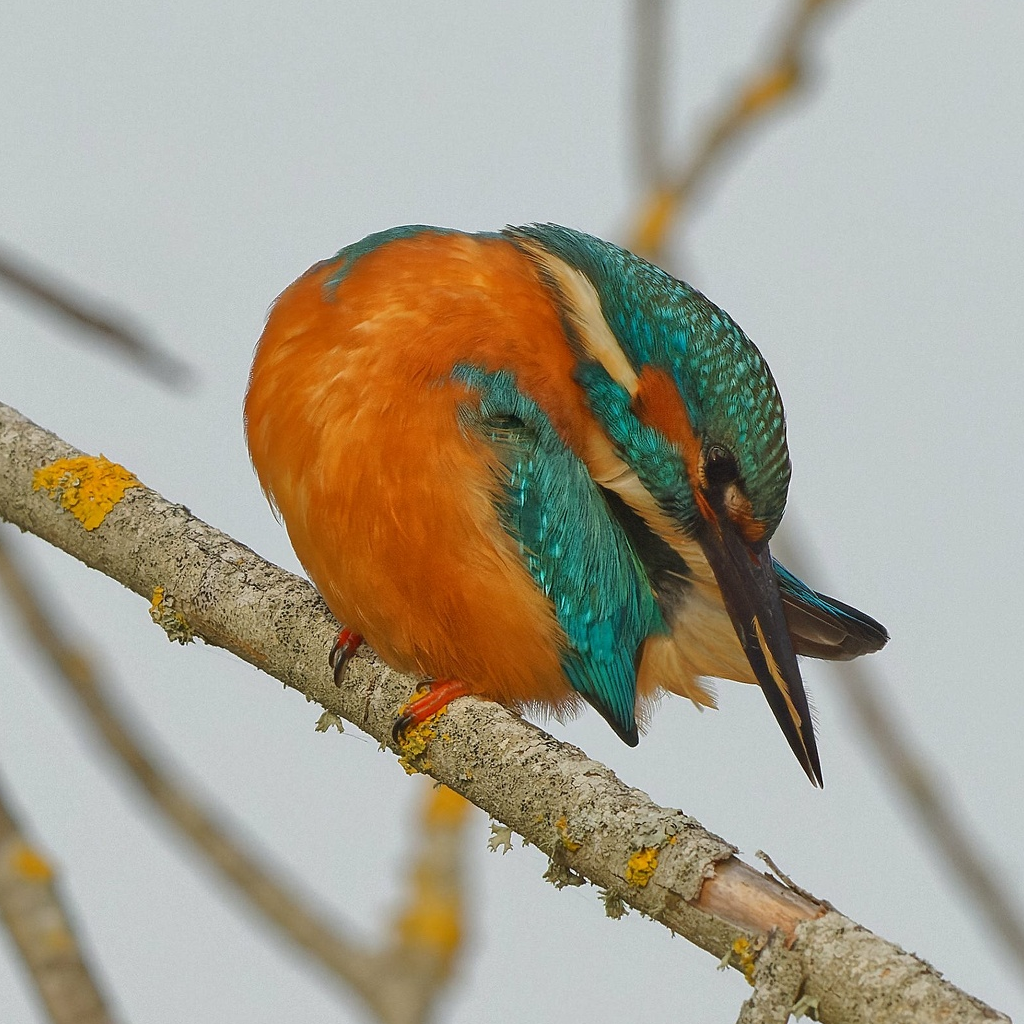
\includegraphics[scale=0.2]{martin_pecheur.png}
\caption{Ceci est un martin pêcheur.}
\label{martin_pecheur}
\end{figure}
\end{verbatim}
\noindent donnera :\\

\begin{figure}[!h]
\centering
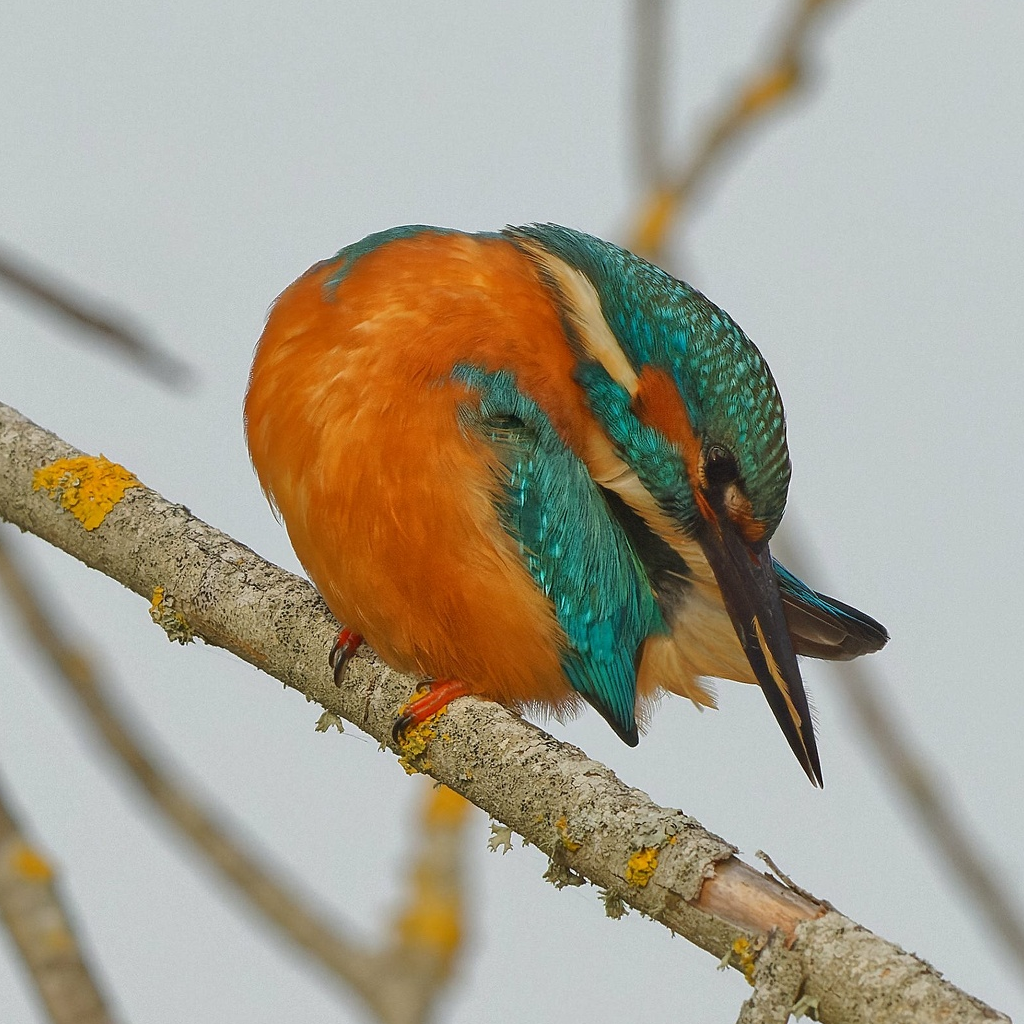
\includegraphics[scale=0.2]{martin_pecheur.png}
\caption{Ceci est un martin pêcheur.}
\label{martin_pecheur}
\end{figure}

On trouve différentes commandes :
\begin{itemize}
\item l'option \verb"!h" permet de placer l'image « ici » (\textit{here}). Sans cette option, l'image sera placée par défaut en haut d'une page (l'actuelle ou la suivante, selon là ou il y a de la place), ce qui peut couper un morceau de texte ou d'environnement ;
\item l'option \verb"\centering" permet de centrer la figure ;
\item \verb"\caption" permet de donner un titre à la figure ;
\item \verb"\label" permet d'ajouter une étiquette pour une référence future (ou passée). Il faut mettre l'étiquette après le titre, pour faire référence au numéro de figure.
\end{itemize}

\subsection{Tracés graphiques}

On présente ici une très brève introduction au tracé graphique, via le paquet \verb"tikz". Très brève, puisque le manuel de Tikz fait 1400 pages, et un manuel d'introduction fait plus de 300 pages. Impossible, donc, de tout présenter en un temps raisonnable. Le plus simple est de procéder par mimétisme en partant d'un graphique existant.

\newpage

\begin{verbatim}
\begin{tikzpicture}[scale=.9] % On peut changer l'échelle de l'image
\draw (1, 2.5) node {$\bullet$}; % Création d'un point
\draw (1, 3) node {Ceci est un point}; % On peut écrire du texte

% On peut tracer des traits
\draw (1, 2.5) -- (3, 1.5); 
% Des rectangles (on indique les coins)
\draw (3, 1.5) rectangle (5, 3); 
% Des cercles (coordonnées du centre avant, rayon après)
\draw (7, 3) circle (1.5);
% Des grilles (on indique les coins) 
\draw (9, 0) grid (13, 5); 
% Des flèches
\draw[->] (13.5, 2.5) -- (15, 3); 

% On peut nommer les points
\node[draw, circle, thick] (A) at (3, 5) {$A$}; 
% On peut utiliser le nom d'un point au lieu des coordonnées
\draw[->, >=stealth] (A) to (5, 4); 
\end{tikzpicture}
\end{verbatim}

\begin{tikzpicture}[scale=.9] % On peut changer l'échelle de l'image
\draw (1, 2.5) node {$\bullet$}; % Création d'un point
\draw (1, 3) node {Ceci est un point}; % On peut écrire du texte

% On peut tracer des traits
\draw (1, 2.5) -- (3, 1.5); 
% Des rectangles (on indique les coins)
\draw (3, 1.5) rectangle (5, 3); 
% Des cercles (coordonnées du centre avant, rayon après)
\draw (7, 3) circle (1.5);
% Des grilles (on indique les coins) 
\draw (9, 0) grid (13, 5); 
% Des flèches
\draw[->] (13.5, 2.5) -- (15, 3); 

% On peut nommer les points
\node[draw, circle, thick] (A) at (3, 5) {$A$}; 
% On peut utiliser le nom d'un point au lieu des coordonnées
\draw[->, >=stealth] (A) to (5, 4); 
\end{tikzpicture}

\begin{verbatim}
% On peut changer les échelles des coordonnées indépendamment
\begin{tikzpicture}[xscale = 1.1, yscale = .5]
% Écriture de boucle
\foreach \x in {0, 3, 5}{
    \draw (\x, 0) node {$\x$};
}

% Le ... permet de compléter automatiquement
\foreach \x in {0, 2, ..., 8}{
    \node[draw, circle] (\x) at (\x, 0.5 * \x + 1) {$\x$};
}

% On peut itérer sur plusieurs variables (mais dans ce cas, on ne
% peut pas utiliser ...)
\foreach \x/\y/\nom in {0/4/A, 3/5/B, 5/3/C}{
    \node[draw, rectangle] (\nom) at (\x, \y) {$\nom$};
}

\foreach \source/\dest in {A/B, B/C}{
    \draw[->, >=latex, very thick] (\source) to (\dest);
}
\end{tikzpicture}
\end{verbatim}

% On peut changer les échelles des coordonnées indépendamment
\begin{tikzpicture}[xscale = 1.1, yscale = .5]
% Écriture de boucle
\foreach \x in {0, 3, 5}{
    \draw (\x, 0) node {$\x$};
}

% Le ... permet de compléter automatiquement
\foreach \x in {0, 2, ..., 8}{
    \node[draw, circle] (\x) at (\x, 0.5 * \x + 1) {$\x$};
}

% On peut itérer sur plusieurs variables (mais dans ce cas, on ne
% peut pas utiliser ...)
\foreach \x/\y/\nom in {0/4/A, 3/5/B, 5/3/C}{
    \node[draw, rectangle] (\nom) at (\x, \y) {$\nom$};
}

\foreach \source/\dest in {A/B, B/C}{
    \draw[->, >=latex, very thick] (\source) to (\dest);
}
\end{tikzpicture}

\begin{verbatim}
% Adapté pour faire des graphes
\begin{tikzpicture}
% On peut créer un type d'objet particulier
\tikzstyle{fleche}=[->,>=latex,thick]
\tikzstyle{sommet}=[draw,circle,minimum size=15pt,inner sep=2pt]
\tikzstyle{carré}=[sommet, rectangle]

% Dès lors, on peut créer les états d'un automate/graphe
\foreach \x/\y/\num/\type in {0/0/0/sommet, 2/2/1/carré, 
                              4/0/2/sommet, 6/0/3/carré}{
    \node[\type] (\num) at (\x, \y) {$q_{\num}$};
}

% On peut faire des arêtes courbées
\draw[fleche] (0) to[bend left] (1);
\draw[fleche] (0) to[bend right] (2);

% Voire choisir les angles de départ et d'arrivée
\draw[fleche] (1) to[out = -90, in = 90] (3);
\end{tikzpicture}
\end{verbatim}

% Adapté pour faire des graphes
\begin{tikzpicture}
% On peut créer un type d'objet particulier
\tikzstyle{fleche}=[->,>=latex,thick]
\tikzstyle{sommet}=[draw,circle,minimum size=15pt,inner sep=2pt]
\tikzstyle{carré}=[sommet, rectangle]

% Dès lors, on peut créer les états d'un graphe
\foreach \x/\y/\num/\type in {0/0/0/sommet, 2/2/1/carré, 
                              4/0/2/sommet, 6/0/3/carré}{
    \node[\type] (\num) at (\x, \y) {$q_{\num}$};
}

% On peut faire des arêtes courbées
\draw[fleche] (0) to[bend left] (1);
\draw[fleche] (0) to[bend right] (2);

% Voire choisir les angles de départ et d'arrivée
\draw[fleche] (1) to[out = -90, in = 90] (3);
\end{tikzpicture}

\begin{verbatim}
% Et pour les automates
\begin{tikzpicture}[->, >=latex, node distance=2.5cm, 
                    initial text=, initial distance=0.5cm, bend angle=35]
\tikzstyle{etat}=[draw,circle,minimum size=15pt,inner sep=2pt]
% initial est un mot clé de la bibliothèque automata
\tikzstyle{init}=[etat, initial] 
\tikzstyle{final}=[etat, double, double distance=2pt]
\tikzstyle{finit}=[init, final]

\node[init] (0) {$q_0$};
\node[finit] (1) [above right of=0] {$q_1$};
\node[etat] (2) [below right of=1] {$q_2$};
\node[final] (3) [right of=2] {$q_3$};

\path
    (0) edge[bend right] node[below] {$a$} (2)
    (0) edge node[near start, left] {$b$} (1)
    (1) edge[out=120, in=60, loop] node[above] {$a,b$} (1)
    (2) edge[bend left] node[above left] {$a$} (3);
\end{tikzpicture}
\end{verbatim}

% Et pour les automates
\begin{tikzpicture}[->, >=latex, node distance=2.5cm, 
                    initial text=, initial distance=0.5cm, bend angle=35]
\tikzstyle{etat}=[draw,circle,minimum size=15pt,inner sep=2pt]
% initial est un mot clé de la bibliothèque automata
\tikzstyle{init}=[etat, initial] 
\tikzstyle{final}=[etat, double, double distance=2pt]
\tikzstyle{finit}=[init, final]

\node[init] (0) {$q_0$};
\node[finit] (1) [above right of=0] {$q_1$};
\node[etat] (2) [below right of=1] {$q_2$};
\node[final] (3) [right of=2] {$q_3$};

\path
    (0) edge[bend right] node[below] {$a$} (2)
    (0) edge node[near start, left] {$b$} (1)
    (1) edge[out=120, in=60, loop] node[above] {$a,b$} (1)
    (2) edge[bend left] node[above left] {$a$} (3);
\end{tikzpicture}

\end{document}